\chapter{\textbf{Introduction}}
\label{ch:intro}

Understanding the origin of the elements has been the primary goal of nuclear astrophysics since its conception. Through the work of Burbidge, Burbidge, Fowler, and Hoyle \cite{Burbidge1957}, it was established that the chemical elements observed in our solar system were synthesized through nuclear burning in stars. Indeed, all but the smallest elements in our observable universe (hydrogen through boron) are the ashes of stellar burning. Consequently, in the quest to discover the nature of the elemental origins, we must understand the nature of stellar processes. From birth to death, stars undergo nuclear reactions in their interiors. With sufficient temperatures, the reaction products themselves undergo subsequent nuclear reactions. An evolutionary stage is reached at which point the star either explodes or otherwise ejects its material outward. This nuclear-processed material is mixed together with the ashes from neighboring stars, forming new stars with new compositions and therefore new nucleosynthesis. One of the most complex evolutionary stages of a star is known as the asymptotic giant branch (AGB) phase, and stars that we currently observe on this phase are known as AGB stars. This thesis focuses on these complex nucleosynthesis processes in massive AGB stars, including s-process nucleosynthesis resulting from thermal pulses, as well as hot-bottom burning at the base of the convective hydrogen envelope. These stellar processes are investigated through laboratory nuclear reaction experiments here on earth. In particular, transfer reaction experiments are used in this thesis as a surrogate for the direct reactions occuring in the stellar processes. These experiments provide information on the nuclear structure of the nuclei involved in the key reactions, and therefore they constrain the reaction rates that are crucial to nucleosynthesis.

The present chapter will provide an overview of the nuclear astrophysics topics addressed in this thesis. Chapter \ref{ch:reactions} will introduce the mathematical formalism for quantifying nucleosynthesis with reaction rates, as well as the formalism for transfer reactions. Chapter \ref{ch:Rb} will address the rubidium overabundance observed in massive AGB stars, as a result of s-process nucleosynthesis. The measurement of the $^{86}\mathrm{Kr}(^{3}\mathrm{He},d)^{87}\mathrm{Rb}$ transfer reaction is proposed to enhance our understanding of the closed-N shell nucleus $^{87}$Rb and its involvement in the rubidium overabundance. Chapter \ref{ch:exp} will introduce the experimental techniques that were used in this thesis to successfully perform transfer reaction experiments. Chapter \ref{ch:DAQ} will introduce the work that was done implementing a new digital data acquisition system (DAQ) for the focal-plane detector package at the Enge Split-Pole Spectrograph, which will replace the current analog system for future transfer reaction experiments. Finally, Chapter \ref{ch:GC} will address the abundance patterns in globular cluster NGC 2419, which may have originated from hot-bottom burning in massive AGB stars. The anomalous Mg--K abundance pattern observed in NGC 2419 is investigated with the $^{39}\mathrm{K}(^{3}\mathrm{He},d)^{40}\mathrm{Ca}$ transfer reaction, and new constraints are placed on the key potassium-destroying reaction $^{39}\mathrm{K}(p,\gamma)^{40}\mathrm{Ca}$ from the first-ever resolution of the 154 keV resonance in $^{39}\mathrm{K}+p$, among the other resonances of astrophysical interest.

\section{AGB Overview}
% Evolution on the H-R diagram (figure). Early (E-AGB) phase versus thermally-pulsing (TP-AGB) phase. The hydrogen and helium burning shells in the TP-AGB phase (with figure). S-Process occuring in the inter-shell region during and between thermal pulses. Hot-bottom burning occuring between the base of the convective hydrogen envelope and the hydrogen-burning shell.
Asymptotic giant branch (AGB) stars produce about half of all elements beyond iron in our galaxy \cite{Busso1999}, and they are one of the leading candidates for the origin of abundance anomalies in globular clusters \cite{Prantzos2007}. An understanding of these stars therefore provides insight into the origin of the elements. AGB stellar evolution is separated into two phases. The \emph{early-AGB} (e-AGB) phase occurs after both hydrogen and helium have been exhausted in the core of a star, leaving behind mostly inert carbon and oxygen. Hydrogen and helium burning is still active in separate shells around the core, with a helium-rich intershell region inbetween. The far more active hydrogen-burning shell perpetually increases the density and temperature of the intershell region, until the rate of energy generated by the helium-burning shell is greater than the rate at which energy can be transported outward through radiative diffusion \cite{Iliadis2015}. A thermal instability, called a \emph{thermal pulse}, occurs as a result, initiating the \emph{thermally pulsing AGB} (TP-AGB) phase, shown in Figure \ref{fig:AGB_Structure}. This pulse causes the helium-burning shell to extend into the intershell region and ignite the hydrogen-burning shell, rendering it inactive for a brief period. The nuclei inside the intershell region get carried outward through the convective envelope toward the surface of the star, where they are ejected into the interstellar medium by stellar winds. The hydrogen-burning shell takes over once again as the dominant energy-producer, and this cycle repeats.

Both during thermal pulses and during the interpulse period, the helium-rich intershell region produces a large flux of neutrons. These neutrons originate from the neutron sources, $^{13}\mathrm{C}(\alpha,n)^{16}\mathrm{O}$ and $^{22}\mathrm{Ne}(\alpha,n)^{25}\mathrm{Mg}$. The former reaction is the dominant neutron source during the interpulse period, where temperatures are between about $100$ MK $\lesssim T \lesssim$ 300 MK and densities are roughly $\rho \approx 10^{7}$ $\mathrm{cm}^{-3}$. During thermal pulses, where $T$ and $\rho$ increase, the latter reaction is dominant and occurs at $T \gtrsim 300$ MK and $\rho \approx 10^{10}$ $\mathrm{cm}^{-3}$. Nucleosynthesis occurs via a series of neutron captures $(n,\gamma)$ and beta decays $\beta^{-}$, known as the (slow) \emph{s-process}, described in Section \ref{sec:s-process}.

In the case of massive AGB stars ($M \gtrsim 4 \, M_{\odot}$), the convective hydrogen envelope reaches down to the top of the hydrogen-burning shell during the interpulse period, where temperatures are at least 50 MK. The resulting hydrogen burning nucleosynthesis is called \emph{hot-bottom burning}, detailed in Section \ref{sec:hot-bottom-burning}, and the products of this burning are brought to the surface by convection.

\begin{figure}[t]
\centering
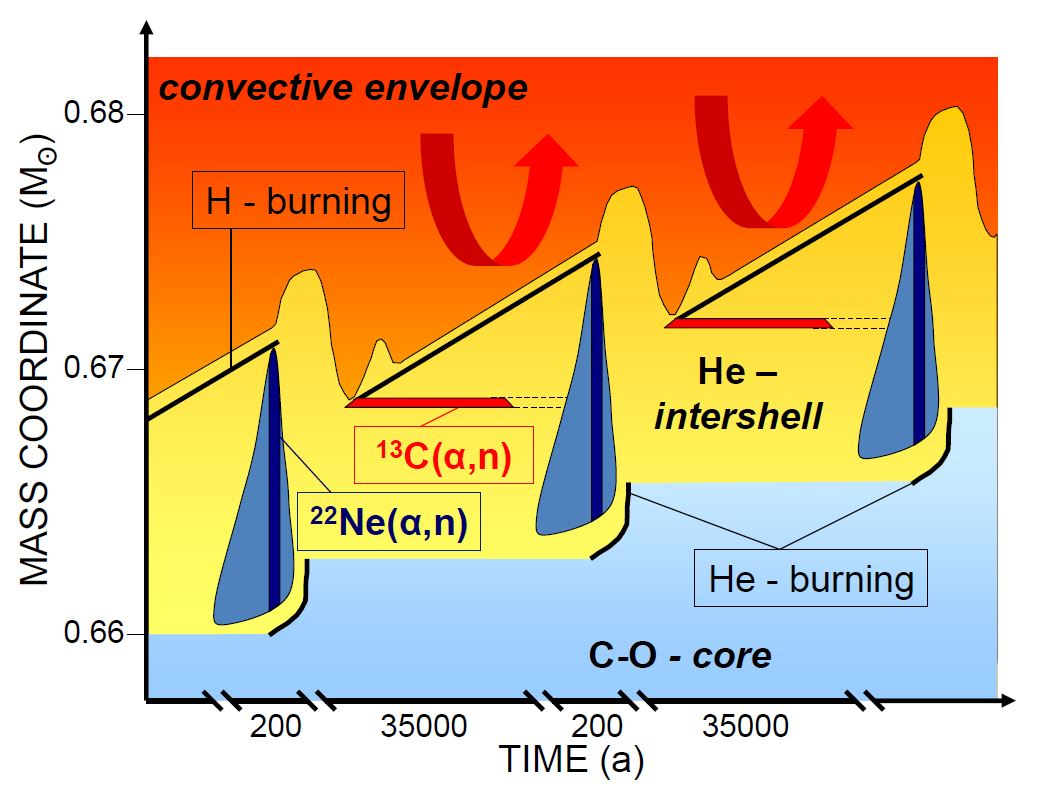
\includegraphics[width=6.5in]{Chapter-1/figs/sProcess_AGB.JPG}
\caption{\label{fig:AGB_Structure}The evolution and structure of a thermally pulsing AGB star. Three thermal pulses are depicted in blue, extinguishing the hydrogen burning shell. The neutron sources $^{13}\mathrm{C}(\alpha,n)^{16}\mathrm{O}$ and $^{22}\mathrm{Ne}(\alpha,n)^{25}\mathrm{Mg}$ are shown to be active between pulses and during pulses, respectively. Figure adapted from Ref. \cite{Reifarth2014}.}
\end{figure}

\section{s-Process Nucleosynthesis} \label{sec:s-process}
% Main and weak components of the s-process here
% s-process paths picture

%Both during thermal pulses and during the interpulse period, the helium-rich intershell region produces a large flux of neutrons. These neutrons originate from the neutron sources, $^{13}\mathrm{C}(\alpha,n)^{16}\mathrm{O}$ and $^{22}\mathrm{Ne}(\alpha,n)^{25}\mathrm{Mg}$. The former reaction is the dominant neutron source during the interpulse period, where temperatures are between about $100$ MK $\lesssim T \lesssim$ 300 MK and densities are roughly $\rho \approx 10^{7}$ $\mathrm{cm}^{-3}$. During thermal pulses, where $T$ and $\rho$ increase, the latter reaction is dominant and occurs at $T \gtrsim 300$ MK and $\rho \approx 10^{10}$ $\mathrm{cm}^{-3}$. Nucleosynthesis occurs via a series of neutron captures $(n,\gamma)$ and beta decays $\beta^{-}$, known as the (slow) \emph{s-process}, described in Section \ref{sec:s-process}.

\subsection{Rubidium Overabundance} \label{subsec:Rb_Overabundance}

% "Rb problem"
% 86Rb branch, 87Rb abundance - connected to 22Ne(a,n)25Mg reaction

\section{Hot-Bottom Burning} \label{sec:hot-bottom-burning}

%In the case of massive AGB stars ($M \gtrsim 4 M_{\odot}$), the convective hydrogen envelope reaches down to the top of the hydrogen-burning shell during the interpulse period, where temperatures are at least 50 MK. The resulting hydrogen burning nucleosynthesis is called \emph{hot-bottom burning}

\subsection{Candidate for Globular Cluster Pollution} \label{subsec:GC_Candidate}

% AGB stars for Prantzos 2007 and Ventura 2012, Super-AGB stars for Illiadis 2016